\section{Evaluation}
 \label{sec:evaluation}
 
 We implemented a prototype of \name in Python. 
 For a given workload, \name outputs Quagga configurations~\cite{quagga}. 
 We use the Gurobi solver~\cite{gurobi} 
 for linear constraints generated by \name.
  In this section, we evaluate \Name using
%\loris{really don't like the word realistic}
enterprise-scale data
center fat-tree topologies~\cite{fattree} of different 
sizes. 
Specifically, we ask the following questions.\footnote{All experiments were conducted using a
32-core Intel-Xeon 2.40GHz CPU machine and
128GB of RAM.}

\vspace{2mm}
\begin{tabular}{p{0.5cm}p{0.88\textwidth}}
\textbf{Q1} &  What is the performance of \name on different synthesis workloads? (\secref{sec:ospfeval})\\

\textbf{Q2} & How resilient are the configurations  generated by \name? (\secref{sec:reseval})\\

\textbf{Q3} &  Can \name get higher resilience when it is allowed to try different domain assignments? (\secref{sec:mcmceval})
\end{tabular}


\subsection{Single Domain End-to-end Performance}\label{sec:ospfeval}


We evaluate the end-to-end performance of our tool
on a  fat-tree 
topology comprising of 45 routers
and a single OSPF domain. 
The size of the topology is consistent with operator preferences to restrict
the size of a domain to under 50 routers (OSPF does not scale
well as domain size increases).
We use PC to refer to the algorithm that handles complex policies and
can synthesize policy-compliant
configurations with few static routes (\secref{sec:config-synthesis})
and 
1-WC (resp. 2-WC) to refer to the version of  the algorithm that handles waypoint policies and
can synthesize policy-compliant
configurations with high policy-resilience starting from 1 path (resp. 2 paths) per waypoint policy (\secref{sec:waypointres}).

We consider two classes of policies.
Our first class contains complex isolation policies that 
existing tools cannot handle; 
for this class we can only 
evaluate algorithm PC.
Our second class consists of
 waypoint policies of the form described in ~\secref{sec:waypointres};
for this class we evaluate 1-WC and 2-WC.
For each algorithm we evaluate how much time is spent 
calling \genesis to generate policy-compliant forwarding paths
and how much time \name takes to generate configurations 
from such paths. 
We set a timeout of 2000 seconds for each workload.


%of the path-compliance synthesis algorithm for tenant 
%isolation workloads, and single-path waypoint-compliance 
%synthesis for varying number of waypoint policies.


\begin{wrapfigure}[14]{r}{0.6\columnwidth}
	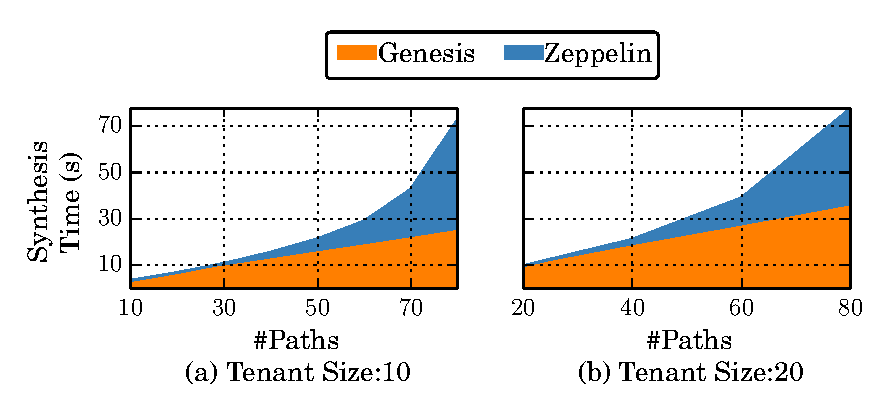
\includegraphics[width=0.58\columnwidth]{figures/ospfisolation.eps}
	%	\subfloat[Number of Route Filters]
	%	{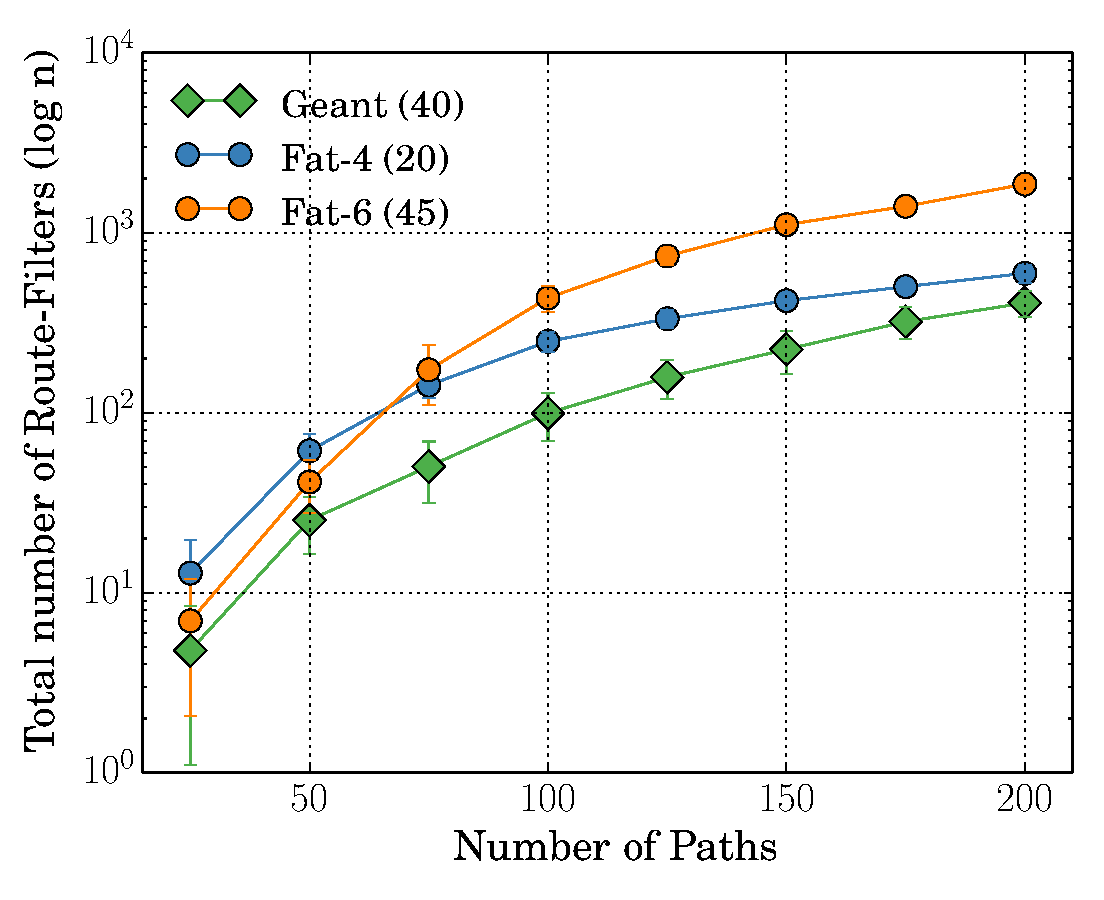
\includegraphics[width=0.33\columnwidth]{figures/ospfRF.eps}}
	%	\subfloat[Endpoint Resilience]
	%	{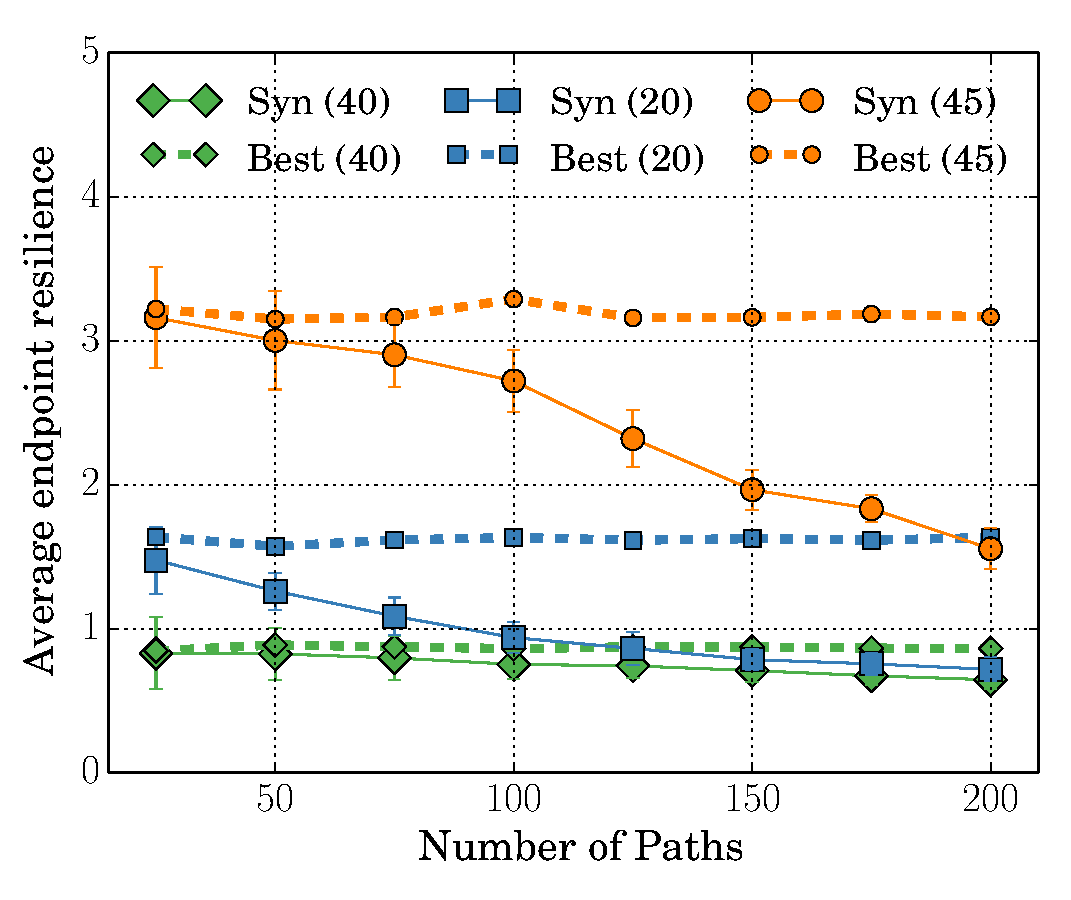
\includegraphics[width=0.32\columnwidth]{figures/ospfAvgRes.eps}}
	\vspace{-8pt}
	\compactcaption{\label{fig:ospfisolation}
		End-to-end synthesis time for isolation workloads over the range of destinations and different tenant sizes.}
\end{wrapfigure}
\paragraph{Isolation Policies.}
We generate policies that operate 
on a multi-tenant topology with 
 different tenants.
Within a  group of tenants, we add a policy to ensure
each path  (with randomly generated endpoints)
is isolated from other paths of the same tenant group.
Here, isolation  prevents interference by other traffic belonging to
same tenant.  
 
For each 
workload, we have $n$ tenant groups (between 1 to 8), 
each group comprised of $g$ destinations (between 10 and 20). 
\Cref{fig:ospfisolation} 
shows the synthesis time 
for PC.
The x-axis shows the number of paths $n * g$ 
to different destination IP addresses. 
 As the number of tenants increase, time to 
synthesize the data plane increases linearly as we only 
consider isolation policies within tenants, not amongst paths 
of different tenants. Meanwhile, time taken to synthesize 
OSPF configurations increases exponentially with increasing 
number of tenants due to the exponential complexity of computing 
the unsat-cores; with increasing number of 
paths, PC needs to add more static routes 
and requires more iterations of the unsat-core learning
procedure. 
For this workload, \name can
synthesize configurations for 4 tenants, each with
20 destinations in 77 seconds, where \genesis takes 35 seconds
for synthesizing paths and synthesizing configurations
takes 42 seconds on average. 


\begin{figure*}
	\begin{center}
		\subfloat[1-WC]
		{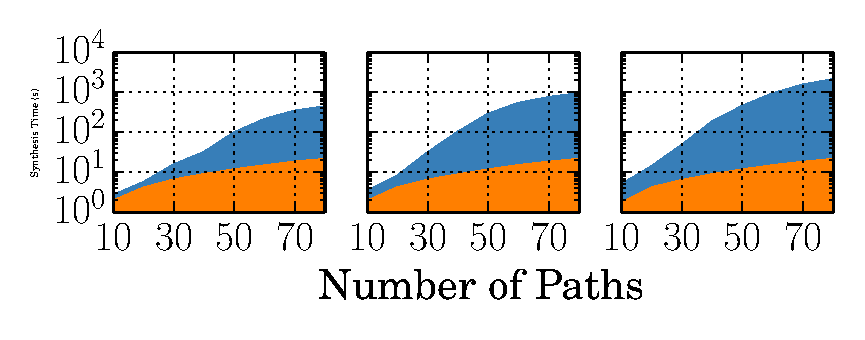
\includegraphics[width=0.5\columnwidth]{figures/ospfwaypoint.eps}}
		\subfloat[2-WC]
		{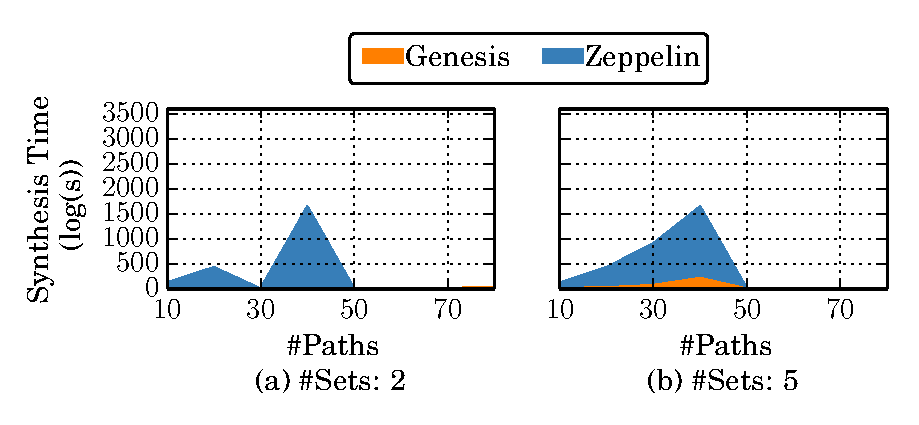
\includegraphics[width=0.5\columnwidth]{figures/ospfwaypoint2.eps}}
		\compactcaption{\label{fig:ospfwaypoint}
			End-to-end synthesis time for waypoint policy workloads for varying 
			number of paths and different number of waypoint sets.}
	\end{center} 
\end{figure*}
\paragraph{Waypoint Policies.}
We generate waypoint policy 
workloads with varying number of destination IP addresses and 
waypoint sets as follows. 
We vary the total number of unique waypoint 
sets to 2 and 5. For each waypoint set, we pick 3 routers randomly.  
Each waypoint set can be 
viewed as a class of replicated middleboxes (e.g., firewalls).
We randomly generate policies that map each destination to one of the waypoint sets. 

%Genesis generates a single path for each 
%destination, and \name synthesizes waypoint-compliant OSPF 
%configurations ((referred to as 1-WC) ) 
%using the waypoint policies and paths generated by Genesis.  

\Cref{fig:ospfwaypoint} shows the end-to-end synthesis
 time for varying number of destination paths and the 
 number of unique waypoint sets (2 and 5). 
 Since synthesizing paths
 for waypoint policies can be done independently,
Genesis synthesis time is small compared to OSPF synthesis. 
\name's 1-WC and 2-WC synthesis 
time increases as we increase the number of waypoint sets,
as we need to add constraints corresponding to $D_s^t(\waypt)$ 
for each set, and thus, computing the unsat-core in each
iteration to find a static route is more expensive with increasing
number of sets. 
For 5 waypoint sets and 40 destinations, \name takes 120 
seconds on average to synthesize waypoint-compliant configurations
and 1800 seconds to synthesize policy-resilient configurations.


In summary, the answer to \textbf{Q1} is that, for realistic workloads,
\textbf{\name can synthesize path-compliant configurations for medium size
topologies} in less than 5 minutes; synthesizing resilient 
configurations is more expensive. 

%\begin{table}{l}{8em}
%	\begin{footnotesize}
%		\begin{center}
%			\begin{tabular}{P{10em}| P{4em} | P{4em} | P{4em} | P{4em}}
%				Synthesis Type & Number of Packet Classes & Avg. Synthesis time (s) & Avg. Number of Resilient Classes & Ratio of Static Routes \\
%				\hline
%				1-Resilient Waypoint & 10 & 122.16 & 7.13 & 7/100\\
%				Waypoint & 10 & 7.85 & 0.3 & 7/100\\
%				1-Resilient Waypoint & 20 & 122.16 & 7.1 & 7/100\\
%				Waypoint & 20 & 7.85 & 0.3 & 7/100\\
%				1-Resilient Waypoint & 40 & 122.16 & 7.1 & 7/100\\
%				Waypoint & 40 & 7.85 & 0.3 & 7/100\\
%			\end{tabular}
%		\end{center}
%		\compactcaption{Average synthesis time per class for waypoint policies with increasing number of waypoints. } \label{tab:waypointeval} 
%	\end{footnotesize}
%\end{table} 

\subsection{Resilience of Synthesized Intra-domain Configurations} \label{sec:reseval}
\paragraph{Connectivity-resilience.}
We measure the connectivity-resilience of the configurations 
generated using the algorithm PC on the isolation workload described in
\secref{sec:ospfeval}. 
For our baseline, we use configurations 
where all the paths synthesized by \genesis
are enforced using only static routes and
OSPF weights are assigned randomly.
\Cref{fig:ospfbaselineresilience}
shows the results. A point above the diagonal 
denotes a benchmark in which \name
generated a configuration with higher connectivity-resilience than
the baseline algorithm.
PC provides an average connectivity-resilience score 
of 0.95 over the baseline score 
of 0.85.
On average, PC places
$(8 \pm 0.5)$\% of the static routes required by the baseline configuration. 


\begin{wrapfigure}{r}{0.20\columnwidth}
	\begin{center}
		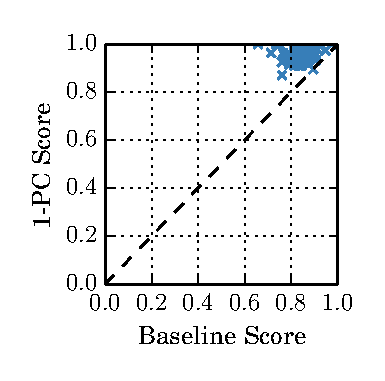
\includegraphics[width=0.20\columnwidth]{figures/ospfbaselineresilience.eps}
		%	\subfloat[Number of Route Filters]
		%	{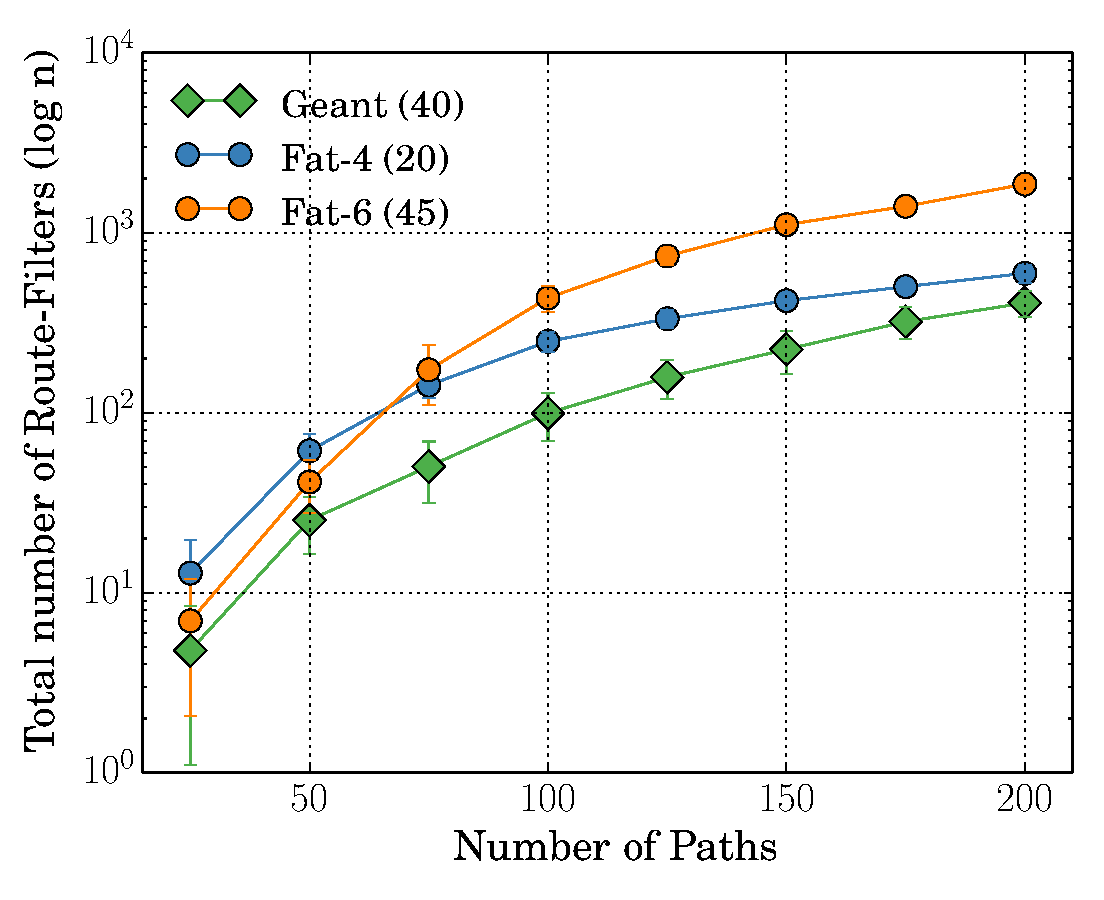
\includegraphics[width=0.33\columnwidth]{figures/ospfRF.eps}}
		%	\subfloat[Endpoint Resilience]
		%	{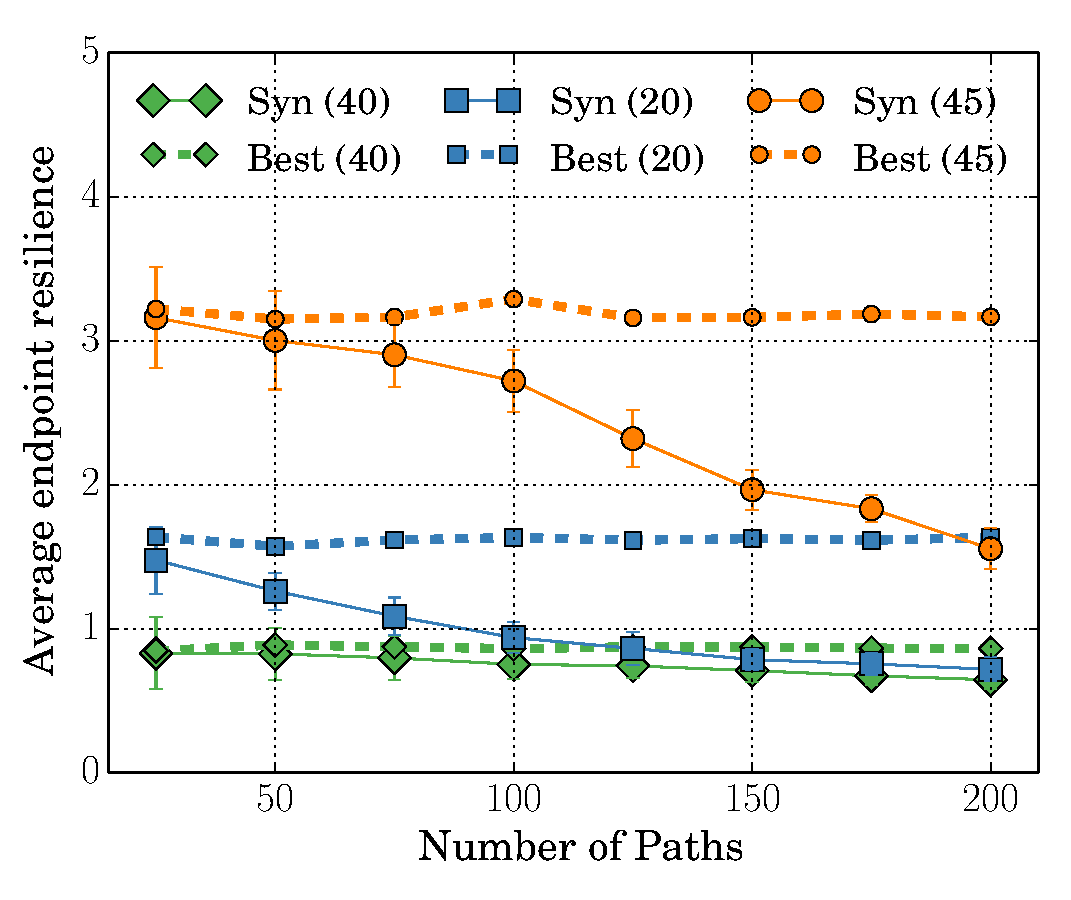
\includegraphics[width=0.32\columnwidth]{figures/ospfAvgRes.eps}}
		\compactcaption{\label{fig:ospfbaselineresilience}
			Connectivity-resilience for 1-PC configurations compared to the baseline 
			configurations.}
	\end{center} 
\end{wrapfigure}


\paragraph{Policy-resilience.}
We measure the policy-resilience of the configurations 
generated using algorithms  1-WC and 2-WC on the waypoint workload described in
\secref{sec:ospfeval} with 5 waypoint sets. 
For each workload, we run each algorithm 
3 times with a different random seed, and report the most-resilient configuration it obtains.
For our baseline, we use the configurations generated by the algorithm PC, which
only tries to reduce the number of placed static routes.

\Cref{fig:ospfbaselineresilience}
shows the results
for varying number of policies (10, 20 and 40), each policy mapped 
to a particular destination IP address. 
For the plot on the left (resp. right)
a point above the diagonal 
denotes a benchmark in which 2-WC
generated a configuration with higher policy-resilience than
PC (resp. 1-WC).
For 40 policies, 
we can observe that 2-WC is able to synthesize 
configurations with high policy-resilience
(average 0.98) over PC (average 0.41) and 1-WC (average 0.51). 
Although not as good as 2-WC, 1-WC is able to provide higher policy-resilience than
1-PC thanks to the relaxed constraints used that do not require
the path given by \genesis to be the shortest one.

\begin{figure*}
	\centering
	\subfloat[2-WC vs. PC]
	{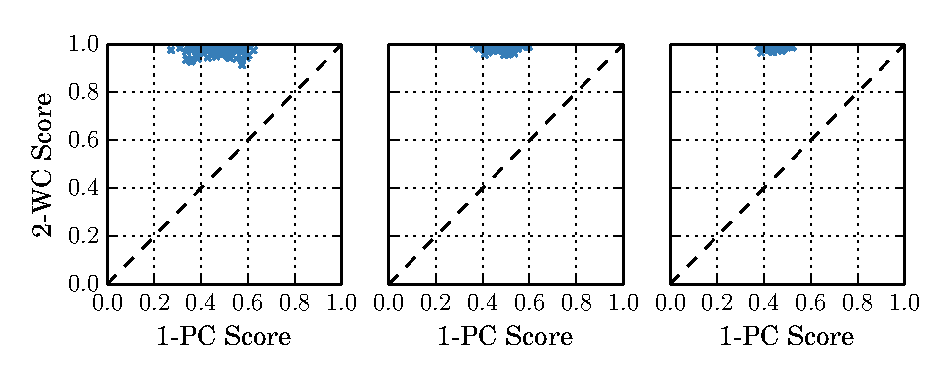
\includegraphics[width=0.49\columnwidth]{figures/ospfresilience2.eps}}
	\subfloat[2-WC vs. 1-WC]
	{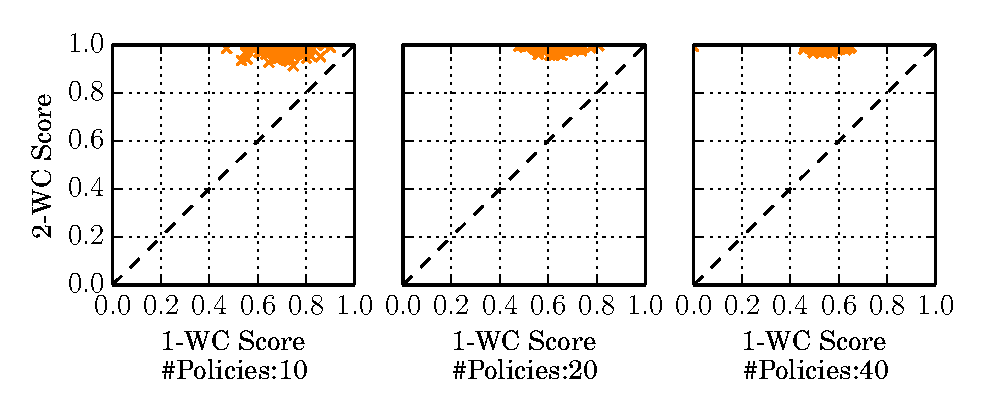
\includegraphics[width=0.5\columnwidth]{figures/ospfresilience.eps}}
	%	\subfloat[Number of Route Filters]
	%	{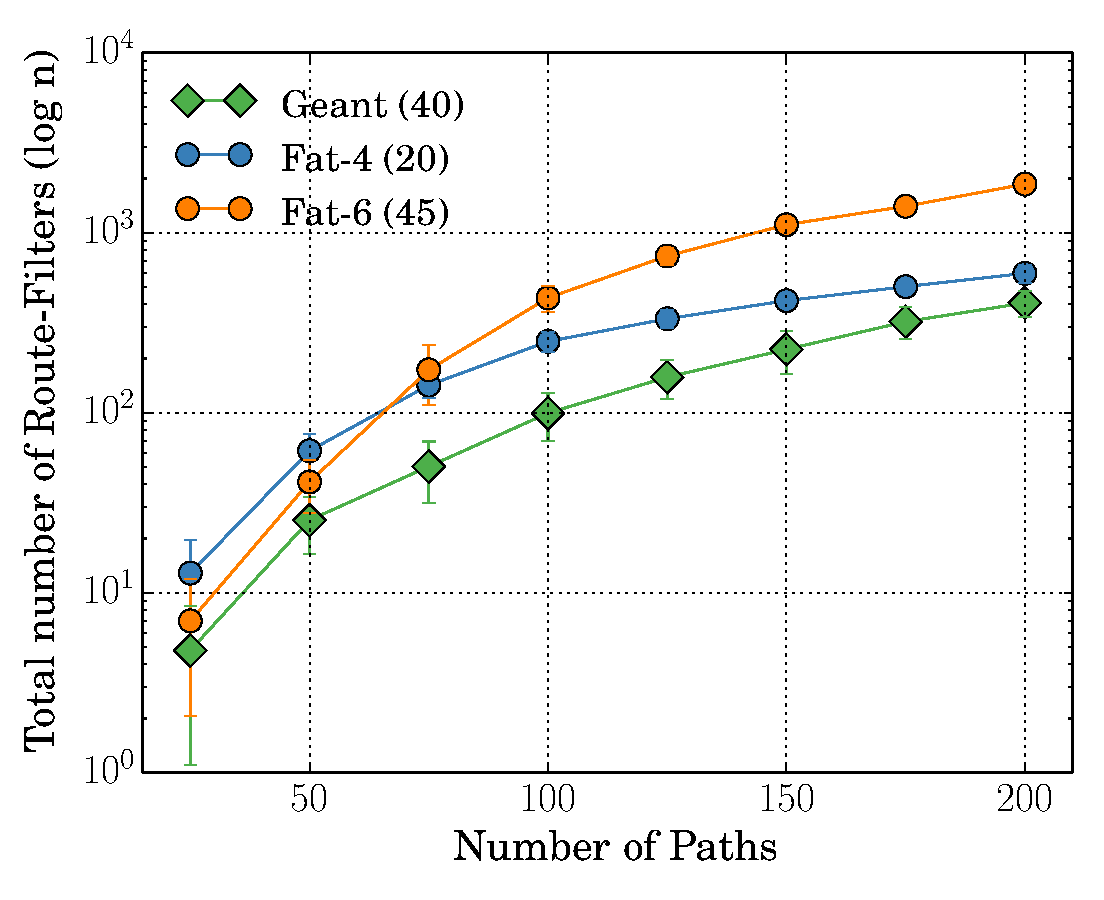
\includegraphics[width=0.33\columnwidth]{figures/ospfRF.eps}}
	%	\subfloat[Endpoint Resilience]
	%	{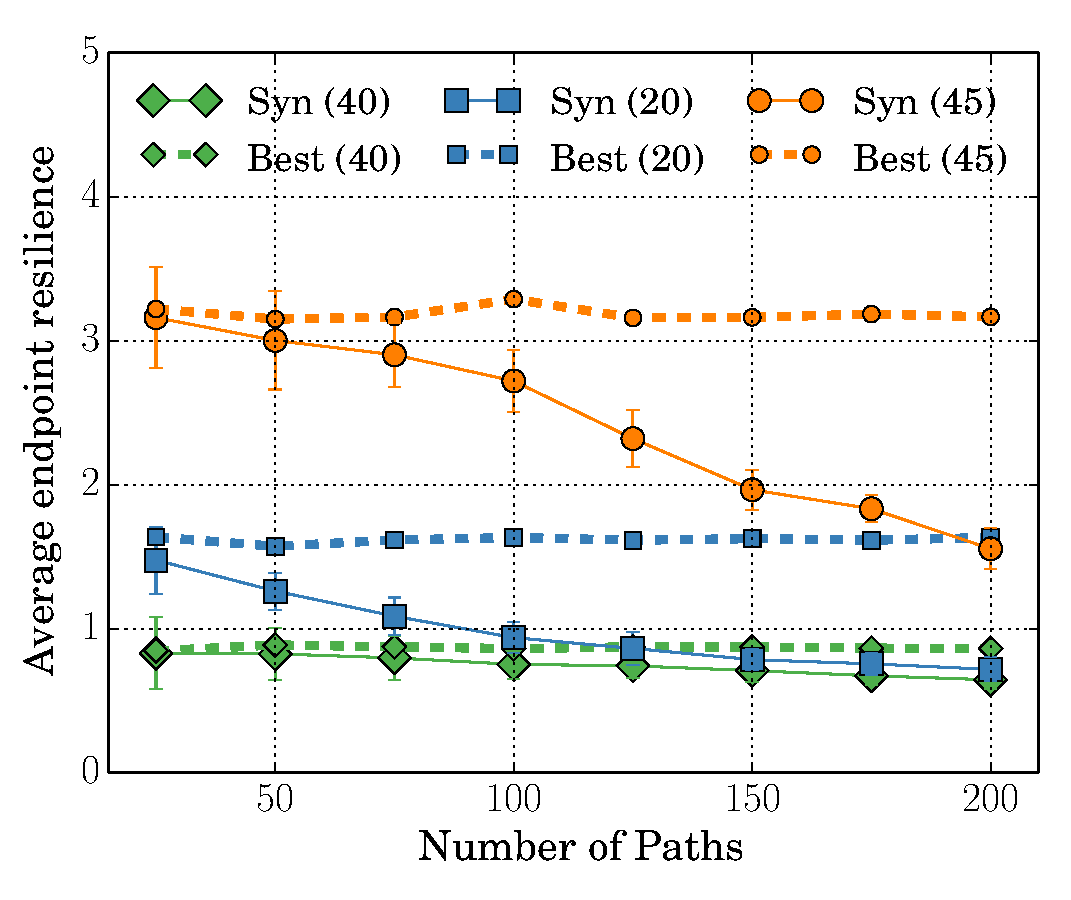
\includegraphics[width=0.32\columnwidth]{figures/ospfAvgRes.eps}}
	\compactcaption{\label{fig:ospfres}
		Policy-resilience scores obtained by 2-WC, 1-WC and PC synthesis 
		for varying waypoint policy workloads.}
\end{figure*}

In summary, the answer to \textbf{Q2} is that
\textbf{\name can synthesize configurations with high resilience} compared to existing approaches.


\subsection{Dynamic Domain Assignment Performance} \label{sec:mcmceval}
\begin{wrapfigure}{r}{0.3\columnwidth}
	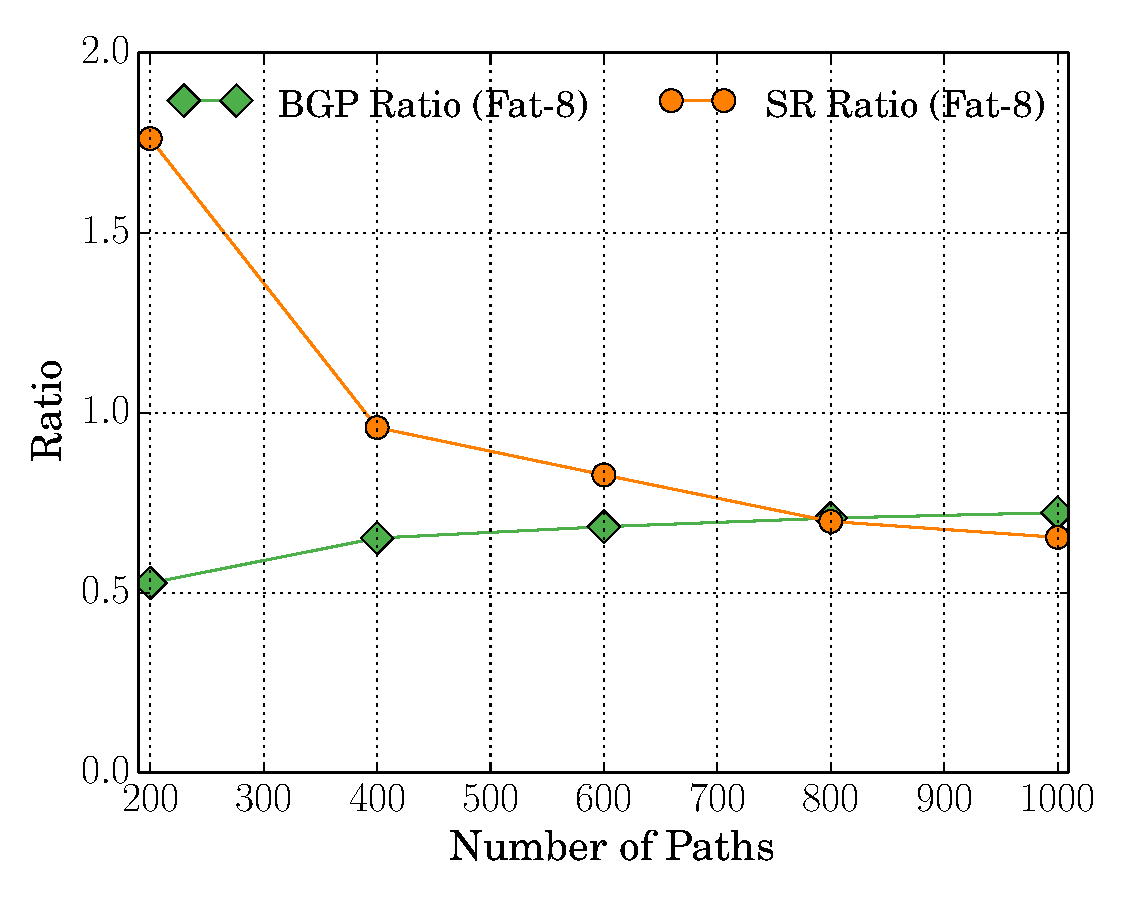
\includegraphics[width=0.29\columnwidth]{figures/ratioMCMC.eps}
	\compactcaption{\label{fig:mcmceval}
		MCMC Evaluation for varying number of paths.}
\end{wrapfigure}

In this section, we measure whether,
useingthe MCMC algorithm presented in \secref{sec:synth-dom-ass}, 
\name can 
generate configurations
with higher resilience when it is allowed to explore different domain assignments.
% the advantages of using MCMC sampling
%to find a domain assignment which can  
%reduce both configuration overhead and number of static routes, 
%leading to higher connectivity-resilience. 
We consider an 80 router fat-tree topology and run the MCMC sampling
for 600s---i.e., more than 100,000 iterations---and the parameter
$\alpha$ that assigns priorities for optimizing configuration overhead
vs static routes is set to 1. For the input, we generate $n$ (between
200 and 1,000) random paths for $n/4$ destination IPs, with random
path length between 3 and 10.  We require \name to split the network
into 5 OSPF domains each with size in range between 4 and 10.

We conduct each experiment 20 times and report averages and standard
deviations.  For each MCMC run, we collect the domain assigments with
worst and best scores.  For these assignments, we use the algorithm PC
to compute path-compliant configurations.
%We also store the worst configuration in terms of either
%configuration overhead $bc$ and the static route cost 
%$sc$. 
\Cref{fig:mcmceval} shows, for varying number of paths, the average ratios
between the best- and worst-score configurations
in terms of
configuration overhead, number of static routes, and 
connectivity-resilience.
For smaller workloads, 
the algorithm reduces the configuration overhead, but increases
the number of static routes, leading to worse connectivity-resilience. For 
larger workloads, the algorithm can
reduce both static routes 
and configuration overhead by $0.3\times$
and improve the connectivity-resilience 
by $0.1\times$.

In summary, the answer to \textbf{Q3} is that,
when allowed to try different domain assignments
\textbf{\name can get configurations with higher connectivity-resilience mainly for workloads with large number of paths}.
